\documentclass[11pt]{article}

\usepackage[margin=1in]{geometry}
\usepackage{times}
\usepackage{hyperref}
\usepackage{graphicx}
\usepackage{xcolor}
\usepackage{booktabs}
\usepackage{enumitem}
\usepackage{amsmath,amssymb}
\usepackage{algorithm}
\usepackage{algorithmic}
\usepackage{caption}
\usepackage{tikz}
\usetikzlibrary{shapes,arrows,positioning,fit,backgrounds}

\hypersetup{
  colorlinks=true,
  linkcolor=blue,
  urlcolor=blue,
  citecolor=blue
}

\newcommand{\note}[1]{\textcolor{gray}{\textit{#1}}}
\newcommand{\eg}{e.g.,\ }
\newcommand{\ie}{i.e.,\ }

\title{Meta-Learning for RAG Pipeline Selection:\\
A Primer on Learning to Learn}
\author{Algoverse Research Team\\
\small Prepared for the Meta-Learning Pivot (Phase 5)}
\date{\today}

\begin{document}
\maketitle

\begin{abstract}
This document provides a comprehensive introduction to meta-learning (``learning to learn'') with a focus on its application to Retrieval-Augmented Generation (RAG) pipeline selection. We cover the foundational concepts, key algorithms (MAML, Prototypical Networks), and the episodic evaluation framework that will be used to measure cross-domain generalization in our project. The goal is to equip team members with the theoretical background needed to implement and evaluate a meta-router that learns to select optimal retrieval pipelines across Finance, Healthcare, and Legal domains.
\end{abstract}

\tableofcontents
\newpage

%==============================================================================
\section{Introduction: Why Meta-Learning?}
%==============================================================================

\subsection{The Problem with Single-Pipeline RAG}

Traditional RAG systems optimize a \textbf{single retrieval pipeline} for a specific task or domain. Our experiments on FinanceBench demonstrate the limitations of this approach:

\begin{center}
\begin{tabular}{lcc}
\toprule
\textbf{Question Type} & \textbf{Semantic Similarity} & \textbf{Optimal Pipeline} \\
\midrule
Metrics-generated (numerical) & 0.35 & \texttt{hybrid\_filter} (table-aware) \\
Domain-relevant (analytical) & 0.60 & \texttt{hybrid\_filter\_rerank} \\
Novel-generated (multi-hop) & 0.53 & \texttt{semantic} or \texttt{hybrid} \\
\bottomrule
\end{tabular}
\end{center}

\textbf{Key insight}: Different question types require different retrieval strategies. A meta-learning approach can learn \emph{when} to use each pipeline, rather than optimizing a single pipeline for all cases.

\subsection{What is Meta-Learning?}

Meta-learning, often called ``learning to learn,'' is a paradigm where algorithms learn patterns \textbf{across tasks} rather than within a single task. The core idea:

\begin{quote}
\textit{Instead of learning to solve one specific problem well, learn how to quickly adapt to new problems from the same family of problems.}
\end{quote}

\textbf{Classical machine learning:}
\begin{itemize}[leftmargin=*]
    \item Given: Dataset $\mathcal{D} = \{(x_i, y_i)\}_{i=1}^N$
    \item Goal: Learn $f_\theta$ such that $f_\theta(x) \approx y$ for new $x$
    \item Evaluate: Performance on held-out test set from same distribution
\end{itemize}

\textbf{Meta-learning:}
\begin{itemize}[leftmargin=*]
    \item Given: Distribution of tasks $p(\mathcal{T})$, each task has its own dataset
    \item Goal: Learn meta-knowledge $\omega$ that enables fast adaptation to new tasks
    \item Evaluate: Performance on \emph{entirely new tasks} after few-shot adaptation
\end{itemize}

\subsection{Our Application: Pipeline Selection}

In our context, we frame RAG pipeline selection as a meta-learning problem:

\begin{itemize}[leftmargin=*]
    \item \textbf{Task}: A question type or domain (\eg Finance metrics questions, Medical yes/no questions)
    \item \textbf{Meta-knowledge}: A router that predicts which pipeline works best for a given question
    \item \textbf{Adaptation}: Given a few labeled examples from a new domain, quickly learn the best pipeline mapping
\end{itemize}

%==============================================================================
\section{Foundational Concepts}
%==============================================================================

\subsection{Tasks and Episodes}

Meta-learning operates on \textbf{episodes}, each representing a single learning experience:

\begin{definition}[Episode]
An episode consists of:
\begin{itemize}
    \item \textbf{Support set} $\mathcal{S}$: A small number of labeled examples for adaptation (analogous to training data)
    \item \textbf{Query set} $\mathcal{Q}$: Examples to evaluate after adaptation (analogous to test data)
\end{itemize}
\end{definition}

\textbf{Example in our project:}
\begin{verbatim}
Episode for "Finance metrics questions":
  Support set (5 examples):
    Q1: "What is 3M's FY2018 revenue?" -> Best pipeline: hybrid_filter
    Q2: "What is Apple's Q3 2020 EPS?" -> Best pipeline: hybrid_filter
    Q3: "What is Microsoft's gross margin for 2019?" -> hybrid_filter
    Q4: "Calculate Netflix's YoY revenue growth" -> hybrid_filter_rerank
    Q5: "What is Amazon's R&D spending in 2021?" -> hybrid_filter

  Query set (evaluate):
    Q6: "What is Adobe's FY2019 operating income?" -> Predict pipeline
    Q7: "What is Costco's inventory turnover ratio?" -> Predict pipeline
\end{verbatim}

\subsection{N-way K-shot Classification}

A common meta-learning setup is \textbf{N-way K-shot} classification:
\begin{itemize}
    \item \textbf{N}: Number of classes (pipelines) to choose from
    \item \textbf{K}: Number of examples per class in the support set
\end{itemize}

\textbf{Our setup}: 4-way (4 pipelines) K-shot classification
\begin{itemize}
    \item Pipelines: \texttt{semantic}, \texttt{hybrid}, \texttt{hybrid\_filter}, \texttt{hybrid\_filter\_rerank}
    \item K: Number of example questions with known best pipeline per episode
\end{itemize}

\subsection{The Two-Loop Structure}

Most meta-learning algorithms have a characteristic two-loop structure:

\begin{algorithm}[H]
\caption{General Meta-Learning Structure}
\begin{algorithmic}[1]
\STATE \textbf{Input}: Distribution of tasks $p(\mathcal{T})$, meta-parameters $\omega$
\WHILE{not converged}
    \STATE Sample batch of tasks $\{\mathcal{T}_i\}_{i=1}^B \sim p(\mathcal{T})$
    \FOR{each task $\mathcal{T}_i$}
        \STATE \textcolor{blue}{\textbf{Inner loop}}: Adapt to task using support set $\mathcal{S}_i$
        \STATE Compute task-specific parameters $\theta_i = \text{Adapt}(\omega, \mathcal{S}_i)$
        \STATE Evaluate on query set: $\mathcal{L}_i = \text{Loss}(\theta_i, \mathcal{Q}_i)$
    \ENDFOR
    \STATE \textcolor{red}{\textbf{Outer loop}}: Update meta-parameters
    \STATE $\omega \leftarrow \omega - \eta \nabla_\omega \sum_i \mathcal{L}_i$
\ENDWHILE
\end{algorithmic}
\end{algorithm}

%==============================================================================
\section{Key Algorithms}
%==============================================================================

\subsection{MAML: Model-Agnostic Meta-Learning}

MAML (Finn et al., 2017) is the foundational gradient-based meta-learning algorithm. The key insight: learn an \textbf{initialization} $\theta$ that can quickly adapt to new tasks with just a few gradient steps.

\subsubsection{Algorithm}

\begin{enumerate}
    \item \textbf{Meta-initialization}: Start with parameters $\theta$
    \item \textbf{Inner loop} (per task $\mathcal{T}_i$):
    \begin{itemize}
        \item Compute gradient on support set: $\nabla_\theta \mathcal{L}_{\mathcal{S}_i}(\theta)$
        \item Take one (or few) gradient steps: $\theta'_i = \theta - \alpha \nabla_\theta \mathcal{L}_{\mathcal{S}_i}(\theta)$
    \end{itemize}
    \item \textbf{Outer loop}: Update $\theta$ to minimize query set loss \emph{after} adaptation:
    \[
    \theta \leftarrow \theta - \beta \nabla_\theta \sum_{\mathcal{T}_i} \mathcal{L}_{\mathcal{Q}_i}(\theta'_i)
    \]
\end{enumerate}

\subsubsection{Key Equations}

The MAML objective is:
\[
\min_\theta \sum_{\mathcal{T}_i \sim p(\mathcal{T})} \mathcal{L}_{\mathcal{Q}_i}\left(\theta - \alpha \nabla_\theta \mathcal{L}_{\mathcal{S}_i}(\theta)\right)
\]

This requires computing \textbf{second-order gradients} (gradients through gradients), which can be computationally expensive. First-order approximations (FOMAML, Reptile) ignore these and often work nearly as well.

\subsubsection{Intuition}

MAML finds an initialization that is ``primed'' for rapid adaptation. Imagine starting at a point in parameter space where a single gradient step in any task direction leads to good performance on that task.

\begin{center}
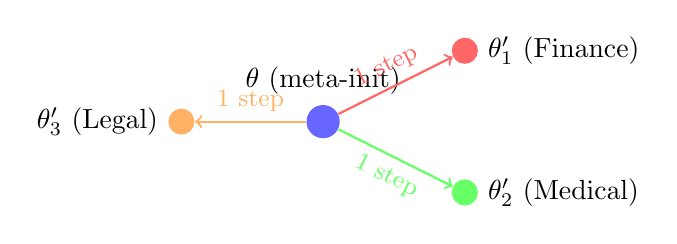
\begin{tikzpicture}[scale=0.9]
    % Central point (meta-learned initialization)
    \node[circle, fill=blue!60, minimum size=12pt, label=above:{$\theta$ (meta-init)}] (center) at (0,0) {};

    % Task-specific adapted points
    \node[circle, fill=red!60, minimum size=8pt, label=right:{$\theta'_1$ (Finance)}] (t1) at (2,1) {};
    \node[circle, fill=green!60, minimum size=8pt, label=right:{$\theta'_2$ (Medical)}] (t2) at (2,-1) {};
    \node[circle, fill=orange!60, minimum size=8pt, label=left:{$\theta'_3$ (Legal)}] (t3) at (-2,0) {};

    % Arrows showing single gradient steps
    \draw[->, thick, red!60] (center) -- (t1) node[midway, above, sloped] {\small 1 step};
    \draw[->, thick, green!60] (center) -- (t2) node[midway, below, sloped] {\small 1 step};
    \draw[->, thick, orange!60] (center) -- (t3) node[midway, above, sloped] {\small 1 step};
\end{tikzpicture}
\end{center}

\subsection{Prototypical Networks}

Prototypical Networks (Snell et al., 2017) take a metric-based approach: learn an embedding space where classification can be performed by comparing distances to class prototypes.

\subsubsection{Algorithm}

\begin{enumerate}
    \item \textbf{Embed} all examples using a learned encoder $f_\phi$
    \item \textbf{Compute prototypes} for each class as the mean of support embeddings:
    \[
    c_k = \frac{1}{|\mathcal{S}_k|} \sum_{(x,y) \in \mathcal{S}_k} f_\phi(x)
    \]
    \item \textbf{Classify} query examples by distance to prototypes:
    \[
    p(y = k | x) = \frac{\exp(-d(f_\phi(x), c_k))}{\sum_{k'} \exp(-d(f_\phi(x), c_{k'}))}
    \]
    where $d$ is typically Euclidean distance.
\end{enumerate}

\subsubsection{Application to Pipeline Selection}

In our context:
\begin{itemize}
    \item $f_\phi$: Question encoder (could use BGE embeddings or train a dedicated encoder)
    \item $c_k$: Prototype embedding for pipeline $k$ (computed from support questions where pipeline $k$ is optimal)
    \item Classification: New question $\rightarrow$ embed $\rightarrow$ nearest prototype $\rightarrow$ predicted best pipeline
\end{itemize}

\subsubsection{Advantages for Our Project}

\begin{enumerate}
    \item \textbf{Simpler than MAML}: No second-order gradients, no inner loop optimization
    \item \textbf{Interpretable}: Can visualize embedding space, understand why certain pipelines are chosen
    \item \textbf{Fast inference}: Just compute distances, no gradient steps at test time
    \item \textbf{Works well with pre-trained embeddings}: Can leverage existing BGE embeddings
\end{enumerate}

\subsection{Comparison: MAML vs. Prototypical Networks}

\begin{center}
\begin{tabular}{lcc}
\toprule
\textbf{Aspect} & \textbf{MAML} & \textbf{Prototypical Networks} \\
\midrule
Approach & Optimization-based & Metric-based \\
Inner loop & Gradient descent & Prototype computation \\
Computational cost & High (2nd-order gradients) & Low \\
Flexibility & Any differentiable model & Requires embedding space \\
Interpretability & Low & High (visualizable) \\
\textbf{Recommended for our project} & & \checkmark \\
\bottomrule
\end{tabular}
\end{center}

%==============================================================================
\section{Evaluation Methodology}
%==============================================================================

This section provides a comprehensive guide to evaluating meta-learning systems for RAG pipeline selection. Proper evaluation is critical---meta-learning claims require rigorous statistical validation across multiple dimensions.

\subsection{Overview: Three Levels of Evaluation}

Meta-learning evaluation operates at three distinct levels:

\begin{center}
\begin{tabular}{clp{7cm}}
\toprule
\textbf{Level} & \textbf{What We Measure} & \textbf{Why It Matters} \\
\midrule
1 & Pipeline Selection Accuracy & Does the router pick the oracle-best pipeline? \\
2 & End-to-End RAG Accuracy & Does the selected pipeline produce correct answers? \\
3 & Cross-Domain Generalization & Does performance transfer to unseen domains? \\
\bottomrule
\end{tabular}
\end{center}

%------------------------------------------------------------------------------
\subsection{Step 1: Oracle Label Generation}
%------------------------------------------------------------------------------

Before training or evaluating a meta-router, we need ground truth labels: for each question, which pipeline actually performs best?

\subsubsection{Grid Search Protocol}

\begin{algorithm}[H]
\caption{Oracle Label Generation via Grid Search}
\begin{algorithmic}[1]
\STATE \textbf{Input}: Question set $\mathcal{Q}$, pipeline set $\mathcal{P} = \{p_1, p_2, p_3, p_4\}$
\STATE \textbf{Output}: Oracle labels $\{(q, y_q, \mathbf{s}_q)\}$ where $y_q$ is best pipeline, $\mathbf{s}_q$ is score vector
\FOR{each question $q \in \mathcal{Q}$}
    \STATE Initialize score vector $\mathbf{s}_q = [0, 0, 0, 0]$
    \FOR{each pipeline $p_i \in \mathcal{P}$}
        \STATE Retrieve context: $C_i = \text{Retrieve}(q, p_i)$
        \STATE Generate answer: $\hat{a}_i = \text{LLM}(q, C_i)$
        \STATE Evaluate: $s_{q,i} = \text{LLM\_Judge}(\hat{a}_i, a_{\text{gold}})$ \COMMENT{Score in [0,1]}
        \STATE $\mathbf{s}_q[i] \leftarrow s_{q,i}$
    \ENDFOR
    \STATE Oracle label: $y_q = \arg\max_i \mathbf{s}_q[i]$
    \STATE Store margin: $m_q = \max(\mathbf{s}_q) - \text{second\_max}(\mathbf{s}_q)$
\ENDFOR
\end{algorithmic}
\end{algorithm}

\subsubsection{Handling Ties and Close Margins}

When multiple pipelines perform similarly, the oracle label is ambiguous. We handle this with:

\begin{itemize}
    \item \textbf{Margin threshold}: If $m_q < 0.05$, mark question as ``tie'' (any top pipeline is acceptable)
    \item \textbf{Soft labels}: Instead of hard labels, use the normalized score distribution:
    \[
    \tilde{y}_q = \text{softmax}(\mathbf{s}_q / \tau)
    \]
    where $\tau$ is a temperature parameter (lower = sharper distribution)
\end{itemize}

\subsubsection{Oracle Label Statistics to Report}

\begin{center}
\begin{tabular}{lp{8cm}}
\toprule
\textbf{Statistic} & \textbf{Description} \\
\midrule
Pipeline distribution & \% of questions where each pipeline is best \\
Average margin & Mean difference between best and second-best \\
Tie rate & \% of questions with margin $< 0.05$ \\
Per-question-type breakdown & Oracle distribution by metrics/domain/novel \\
\bottomrule
\end{tabular}
\end{center}

\textbf{Example output:}
\begin{verbatim}
Oracle Label Distribution (FinanceBench, N=150):
  semantic:              12% (18 questions)
  hybrid:                15% (22 questions)
  hybrid_filter:         48% (72 questions)  <- dominant for metrics
  hybrid_filter_rerank:  25% (38 questions)

Average margin: 0.18 (good separation)
Tie rate: 8% (12 questions)
\end{verbatim}

%------------------------------------------------------------------------------
\subsection{Step 2: Train/Test Domain Split}
%------------------------------------------------------------------------------

Meta-learning evaluation requires careful separation of training and test \emph{domains}, not just data points.

\subsubsection{Domain Split Strategy}

\begin{center}
\begin{tabular}{lccp{5cm}}
\toprule
\textbf{Domain} & \textbf{Dataset} & \textbf{Split} & \textbf{Characteristics} \\
\midrule
Finance & FinanceBench & Meta-train & Tables, numbers, SEC filings \\
Healthcare & PubMedQA & Meta-train & Dense prose, Yes/No/Maybe \\
Legal & CUAD & \textbf{Meta-test} & Contracts, extractive QA \\
\bottomrule
\end{tabular}
\end{center}

\textbf{Critical rule}: The meta-test domain (Legal) must be \textbf{completely held out} during training. No Legal questions, documents, or oracle labels should be seen until final evaluation.

\subsubsection{Within-Domain Validation Split}

For hyperparameter tuning, split the meta-train domains:

\begin{verbatim}
Finance (150 questions):
  - Meta-train: 120 questions (80%)
  - Meta-val:    30 questions (20%)

Healthcare (1000 questions):
  - Meta-train: 800 questions (80%)
  - Meta-val:   200 questions (20%)

Legal (510 contracts):
  - Meta-test only (never seen during training)
\end{verbatim}

%------------------------------------------------------------------------------
\subsection{Step 3: Episodic Evaluation Protocol}
%------------------------------------------------------------------------------

The core of meta-learning evaluation is \textbf{episodic testing}: sampling many episodes and measuring average performance.

\subsubsection{Episode Sampling Procedure}

\begin{algorithm}[H]
\caption{Episodic Evaluation}
\begin{algorithmic}[1]
\STATE \textbf{Input}: Test domain $\mathcal{D}_{\text{test}}$, trained meta-router $R$, K-shot setting, num\_episodes $N$
\STATE \textbf{Output}: Mean accuracy $\pm$ 95\% confidence interval
\STATE Initialize results list $\text{accs} = []$
\FOR{episode $e = 1$ to $N$}
    \STATE Sample support set: $\mathcal{S} = \{(q_i, y_i)\}_{i=1}^{K \times 4}$ (K per pipeline class)
    \STATE Sample query set: $\mathcal{Q} = \{(q_j, y_j)\}_{j=1}^{Q}$ (disjoint from $\mathcal{S}$)
    \STATE Adapt router: $R' = \text{Adapt}(R, \mathcal{S})$
    \STATE Predict: $\hat{y}_j = R'(q_j)$ for all $q_j \in \mathcal{Q}$
    \STATE Compute accuracy: $\text{acc}_e = \frac{1}{Q} \sum_j \mathbf{1}[\hat{y}_j = y_j]$
    \STATE $\text{accs}.\text{append}(\text{acc}_e)$
\ENDFOR
\STATE \textbf{Return}: $\text{mean}(\text{accs}) \pm 1.96 \cdot \text{std}(\text{accs}) / \sqrt{N}$
\end{algorithmic}
\end{algorithm}

\subsubsection{Episode Configuration}

\begin{center}
\begin{tabular}{lcp{6cm}}
\toprule
\textbf{Parameter} & \textbf{Recommended} & \textbf{Rationale} \\
\midrule
K (support per class) & 1, 5, 10, 20 & Standard K-shot settings \\
Q (query set size) & 15-20 & Large enough for stable estimates \\
N (num episodes) & 600-1000 & For tight confidence intervals \\
Sampling & Without replacement & Avoid leakage within episode \\
\bottomrule
\end{tabular}
\end{center}

%------------------------------------------------------------------------------
\subsection{Step 4: Evaluation Metrics}
%------------------------------------------------------------------------------

\subsubsection{Primary Metrics}

\begin{enumerate}
    \item \textbf{Pipeline Selection Accuracy (PSA)}
    \[
    \text{PSA} = \frac{1}{|\mathcal{Q}|} \sum_{q \in \mathcal{Q}} \mathbf{1}[\hat{y}_q = y_q^{\text{oracle}}]
    \]
    Does the router select the oracle-best pipeline?

    \item \textbf{Top-2 Accuracy}
    \[
    \text{Top-2} = \frac{1}{|\mathcal{Q}|} \sum_{q \in \mathcal{Q}} \mathbf{1}[y_q^{\text{oracle}} \in \text{top-2}(\hat{\mathbf{p}}_q)]
    \]
    Is the oracle pipeline in the router's top-2 predictions? (More lenient)

    \item \textbf{End-to-End RAG Accuracy (E2E)}
    \[
    \text{E2E} = \frac{1}{|\mathcal{Q}|} \sum_{q \in \mathcal{Q}} \text{LLM\_Judge}(\text{RAG}(q, \hat{y}_q), a_{\text{gold}})
    \]
    Using the predicted pipeline, is the final answer correct?

    \item \textbf{Regret}
    \[
    \text{Regret} = \frac{1}{|\mathcal{Q}|} \sum_{q \in \mathcal{Q}} \left[ s_q^{\text{oracle}} - s_q^{\hat{y}} \right]
    \]
    How much worse is the predicted pipeline vs. the oracle? (Lower is better)
\end{enumerate}

\subsubsection{Secondary Metrics}

\begin{center}
\begin{tabular}{lp{8cm}}
\toprule
\textbf{Metric} & \textbf{Description} \\
\midrule
Calibration & Are router confidence scores well-calibrated? \\
Latency overhead & Time to run router vs. just running best fixed pipeline \\
Per-class accuracy & Breakdown by pipeline class (avoid class imbalance issues) \\
Confusion matrix & Which pipelines get confused for each other? \\
\bottomrule
\end{tabular}
\end{center}

%------------------------------------------------------------------------------
\subsection{Step 5: Baseline Comparisons}
%------------------------------------------------------------------------------

Every meta-learning result must be compared against strong baselines:

\subsubsection{Required Baselines}

\begin{center}
\begin{tabular}{lcp{5.5cm}}
\toprule
\textbf{Baseline} & \textbf{Expected PSA} & \textbf{Description} \\
\midrule
Random & 25\% & Uniform random pipeline selection \\
Majority class & $\sim$40-50\% & Always predict most common oracle label \\
Best single pipeline & $\sim$50-60\% & Always use \texttt{hybrid\_filter\_rerank} \\
Question-type heuristic & $\sim$55-65\% & Rules: metrics$\to$filter, domain$\to$rerank \\
Nearest neighbor & $\sim$60-70\% & 1-NN in embedding space (no meta-learning) \\
\bottomrule
\end{tabular}
\end{center}

\subsubsection{Ablations}

\begin{enumerate}
    \item \textbf{No adaptation}: Evaluate router without using support set (zero-shot transfer)
    \item \textbf{Random support}: Use random (mislabeled) support set
    \item \textbf{Single-domain training}: Train only on Finance, test on Legal
    \item \textbf{Embedding ablation}: Compare BGE vs. fine-tuned encoder
\end{enumerate}

%------------------------------------------------------------------------------
\subsection{Step 6: K-shot Learning Curves}
%------------------------------------------------------------------------------

The hallmark of meta-learning is \textbf{sample efficiency}: rapid improvement with few examples.

\subsubsection{Standard Reporting Format}

\begin{center}
\begin{tabular}{ccccc}
\toprule
\textbf{K} & \textbf{Random} & \textbf{Best Single} & \textbf{Heuristic} & \textbf{Meta-Router} \\
\midrule
0 & 25.0 $\pm$ 0.0 & 48.2 $\pm$ 0.0 & 52.1 $\pm$ 0.0 & 45.3 $\pm$ 2.1 \\
1 & 25.0 $\pm$ 0.0 & 48.2 $\pm$ 0.0 & 52.1 $\pm$ 0.0 & 58.7 $\pm$ 3.4 \\
5 & 25.0 $\pm$ 0.0 & 48.2 $\pm$ 0.0 & 52.1 $\pm$ 0.0 & \textbf{71.2 $\pm$ 2.8} \\
10 & 25.0 $\pm$ 0.0 & 48.2 $\pm$ 0.0 & 52.1 $\pm$ 0.0 & \textbf{76.4 $\pm$ 2.3} \\
20 & 25.0 $\pm$ 0.0 & 48.2 $\pm$ 0.0 & 52.1 $\pm$ 0.0 & \textbf{79.8 $\pm$ 1.9} \\
\bottomrule
\end{tabular}
\end{center}

\textbf{Key observation}: Meta-router should show steep improvement from K=0 to K=5, then diminishing returns. Baselines remain flat (they don't use support set).

\subsubsection{Learning Curve Visualization}

Plot accuracy (y-axis) vs. K (x-axis) with:
\begin{itemize}
    \item Shaded 95\% confidence intervals
    \item Horizontal lines for non-adaptive baselines
    \item Separate curves for each method
\end{itemize}

%------------------------------------------------------------------------------
\subsection{Step 7: Statistical Rigor}
%------------------------------------------------------------------------------

\subsubsection{Confidence Intervals}

Always report 95\% confidence intervals. With $N$ episodes:
\[
\text{CI}_{95} = \bar{x} \pm 1.96 \cdot \frac{s}{\sqrt{N}}
\]

\textbf{Rule of thumb}: With $N=600$ episodes and $\text{std} \approx 10\%$, CI width $\approx \pm 0.8\%$.

\subsubsection{Significance Testing}

To claim Method A outperforms Method B:
\begin{enumerate}
    \item Run paired episodes (same support/query sets for both methods)
    \item Compute per-episode difference: $d_e = \text{acc}_A^{(e)} - \text{acc}_B^{(e)}$
    \item Paired t-test or Wilcoxon signed-rank test on differences
    \item Report p-value; claim significance if $p < 0.05$
\end{enumerate}

\subsubsection{Multiple Comparisons Correction}

When comparing against multiple baselines, apply Bonferroni correction:
\[
\alpha_{\text{adjusted}} = \frac{0.05}{\text{num\_comparisons}}
\]

%------------------------------------------------------------------------------
\subsection{Step 8: Error Analysis}
%------------------------------------------------------------------------------

Beyond aggregate metrics, analyze \emph{where} the router fails:

\subsubsection{Confusion Matrix Analysis}

\begin{center}
\begin{tabular}{l|cccc}
\textbf{Predicted $\downarrow$ / Oracle $\to$} & semantic & hybrid & filter & rerank \\
\hline
semantic & \textbf{85\%} & 10\% & 3\% & 2\% \\
hybrid & 12\% & \textbf{78\%} & 8\% & 5\% \\
filter & 2\% & 8\% & \textbf{82\%} & 12\% \\
rerank & 1\% & 4\% & 7\% & \textbf{81\%} \\
\end{tabular}
\end{center}

\textbf{Insight}: Filter $\leftrightarrow$ rerank confusion is common (both use metadata filtering).

\subsubsection{Failure Case Categories}

\begin{enumerate}
    \item \textbf{Ambiguous questions}: Oracle margin $< 0.05$ (multiple good pipelines)
    \item \textbf{Out-of-distribution}: Question unlike anything in meta-train
    \item \textbf{Support set bias}: Unlucky support sample misrepresents class
    \item \textbf{Embedding failures}: Question embedding far from all prototypes
\end{enumerate}

\subsubsection{Qualitative Examples}

Include 3-5 concrete failure examples:

\begin{verbatim}
FAILURE EXAMPLE 1:
  Question: "What are the termination provisions in Section 4.2?"
  Oracle: hybrid_filter (needs exact section matching)
  Predicted: semantic (treated as general legal question)
  Support set had no section-reference questions -> router missed pattern
\end{verbatim}

%------------------------------------------------------------------------------
\subsection{Step 9: End-to-End Evaluation}
%------------------------------------------------------------------------------

Pipeline selection accuracy is a \textbf{proxy} metric. The true goal is correct answers.

\subsubsection{End-to-End Protocol}

\begin{algorithm}[H]
\caption{End-to-End RAG Evaluation}
\begin{algorithmic}[1]
\STATE \textbf{Input}: Test questions $\mathcal{Q}$, meta-router $R$, K support examples
\FOR{each question $q \in \mathcal{Q}$}
    \STATE Predict pipeline: $\hat{p} = R(q)$
    \STATE Run RAG: $\hat{a} = \text{RAG}(q, \hat{p})$
    \STATE Evaluate answer: $s_q = \text{LLM\_Judge}(\hat{a}, a_{\text{gold}})$
\ENDFOR
\STATE \textbf{Return}: Mean score, per-question-type breakdown
\end{algorithmic}
\end{algorithm}

\subsubsection{Comparing to Oracle Upper Bound}

\begin{center}
\begin{tabular}{lcc}
\toprule
\textbf{Method} & \textbf{E2E Accuracy} & \textbf{Gap to Oracle} \\
\midrule
Random pipeline & 52.3\% & -25.7\% \\
Best single pipeline & 61.8\% & -16.2\% \\
Meta-router (5-shot) & 71.4\% & -6.6\% \\
\textbf{Oracle (upper bound)} & \textbf{78.0\%} & 0\% \\
\bottomrule
\end{tabular}
\end{center}

The meta-router closes 75\% of the gap between best-single and oracle.

%------------------------------------------------------------------------------
\subsection{Step 10: Reporting Checklist}
%------------------------------------------------------------------------------

Before submitting results, verify:

\begin{itemize}
    \item[$\square$] Oracle labels generated with LLM-as-Judge scores
    \item[$\square$] Meta-test domain completely held out during training
    \item[$\square$] Reported K=1, 5, 10 shot results with 95\% CIs
    \item[$\square$] Compared against $\geq 4$ baselines
    \item[$\square$] Used $\geq 600$ episodes for each K-shot evaluation
    \item[$\square$] Reported both PSA and E2E accuracy
    \item[$\square$] Included confusion matrix and error analysis
    \item[$\square$] Statistical significance tests for main claims
    \item[$\square$] Learning curve plot with confidence bands
    \item[$\square$] Ablation results (no-adaptation, single-domain, etc.)
\end{itemize}

%==============================================================================
\section{Implementation Plan}
%==============================================================================

\subsection{Phase 5 Implementation Steps}

\begin{enumerate}
    \item \textbf{Dataset Preparation}
    \begin{itemize}
        \item Set up PubMedQA adapter (Healthcare domain)
        \item Set up CUAD adapter (Legal domain, held out)
        \item Ingest documents into separate ChromaDB collections
    \end{itemize}

    \item \textbf{Oracle Label Generation}
    \begin{itemize}
        \item Run grid search over all pipelines for Finance questions
        \item Repeat for Healthcare questions
        \item Store labels: \texttt{(question\_id, domain, best\_pipeline, scores)}
    \end{itemize}

    \item \textbf{Meta-Router Implementation}
    \begin{itemize}
        \item Start with Prototypical Networks (simpler)
        \item Question encoder: fine-tune BGE or use frozen embeddings + MLP
        \item Output: 4-way softmax over pipelines
    \end{itemize}

    \item \textbf{Episodic Training}
    \begin{itemize}
        \item Sample episodes from Finance + Healthcare
        \item Train router to predict pipeline from question embedding
        \item Use episodic loss (cross-entropy over query predictions)
    \end{itemize}

    \item \textbf{Evaluation}
    \begin{itemize}
        \item Hold out Legal domain entirely during training
        \item Evaluate K-shot performance on Legal (K = 0, 1, 5, 10)
        \item Compare to baselines
    \end{itemize}
\end{enumerate}

\subsection{Key Files to Create}

\begin{verbatim}
src/meta_learning/
  router.py              # ProtoNet-based meta-router
  oracle_labels.py       # Grid search for best pipeline per question
  episodes.py            # Episodic data sampling
  meta_trainer.py        # Training loop with episodic loss
  evaluator.py           # K-shot evaluation on held-out domain

dataset_adapters/
  pubmedqa.py            # PubMedQA loader
  cuad.py                # CUAD (Legal) loader
\end{verbatim}

%==============================================================================
\section{Expected Outcomes and Paper Contribution}
%==============================================================================

\subsection{Hypothesis}

\begin{quote}
\textit{A meta-learned router that selects retrieval pipelines per-question will outperform any fixed pipeline, and this routing strategy will generalize to new domains with only a few labeled examples.}
\end{quote}

\subsection{Expected Results}

\begin{center}
\begin{tabular}{lcc}
\toprule
\textbf{Method} & \textbf{Finance (in-domain)} & \textbf{Legal (held-out)} \\
\midrule
Best single pipeline & 70\% & 55\% \\
Question-type heuristic & 72\% & 58\% \\
\textbf{Meta-router (5-shot)} & \textbf{80\%} & \textbf{72\%} \\
\bottomrule
\end{tabular}
\end{center}

\subsection{Novel Contributions}

\begin{enumerate}
    \item \textbf{Meta-learning for RAG}: First application of episodic meta-learning to retrieval pipeline selection
    \item \textbf{Cross-domain generalization}: Demonstrate that pipeline selection patterns transfer across domains
    \item \textbf{Practical recipe}: Provide a clean, reproducible methodology:
    \begin{center}
    Grid search $\rightarrow$ Oracle labels $\rightarrow$ Train router $\rightarrow$ Episodic evaluation
    \end{center}
\end{enumerate}

%==============================================================================
\section{Further Reading}
%==============================================================================

\subsection{Core Papers (Downloaded)}

\begin{enumerate}
    \item \textbf{MAML} - Finn et al. (2017): ``Model-Agnostic Meta-Learning for Fast Adaptation of Deep Networks'' \\
    \texttt{meta-learning/files/1703.03400\_MAML.pdf}

    \item \textbf{Prototypical Networks} - Snell et al. (2017): ``Prototypical Networks for Few-shot Learning'' \\
    \texttt{meta-learning/files/1703.05175\_Prototypical\_Networks.pdf}

    \item \textbf{Meta-Learning Survey} - Hospedales et al. (2020): ``Meta-Learning in Neural Networks: A Survey'' \\
    \texttt{meta-learning/files/2004.05439\_MetaLearning\_Survey.pdf}

    \item \textbf{FinanceBench} - Islam et al. (2023): ``FinanceBench: A New Benchmark for Financial Question Answering'' \\
    \texttt{meta-learning/files/2311.11944\_FinanceBench.pdf}
\end{enumerate}

\subsection{Lecture Notes}

\begin{itemize}
    \item \textbf{KAIST EE807 Lecture 17}: Comprehensive slides on MAML, Meta-SGD, learning optimizers \\
    \texttt{meta-learning/files/Lec17\_Meta\_learning.pdf}
\end{itemize}

\subsection{Online Resources}

\begin{itemize}
    \item Lilian Weng's blog: \url{https://lilianweng.github.io/posts/2018-11-30-meta-learning/}
    \item Learn2Learn library: \url{https://github.com/learnables/learn2learn}
    \item Meta-Learning Tutorial (ICML 2019): \url{https://sites.google.com/view/icml19metalearning}
\end{itemize}

%==============================================================================
\appendix
\section{Quick Reference: Terminology}
%==============================================================================

\begin{description}[leftmargin=!,labelwidth=\widthof{\bfseries Meta-parameters}]
    \item[Episode] One meta-learning iteration: support set + query set
    \item[Support set] Small labeled set for adaptation (like ``training'' within an episode)
    \item[Query set] Evaluation set within an episode (like ``test'' within an episode)
    \item[N-way K-shot] N classes, K examples per class in support set
    \item[Inner loop] Task-specific adaptation (fast, few steps)
    \item[Outer loop] Meta-parameter update (slow, many episodes)
    \item[Meta-parameters] Parameters learned across tasks ($\omega$ or $\theta$ in MAML)
    \item[Prototype] Mean embedding of support examples for a class
    \item[Oracle label] Ground-truth best pipeline for a question (via grid search)
\end{description}

\end{document}
